%\vspace*{-1ex}
\section{Motivation and Challenges}
\label{sec-2}

In this section, we first motivate the need for on-demand image
retrieval, then describe our approach and illustrate the challenges
facing on-demand image retrieval.

\mypar{Motivation.}
With the increasing penetration of mobile devices with high-resolution
imaging sensors, point-and-shoot cameras and camcorders are
increasingly being replaced by mobile devices for taking photos and
videos.
%
This trend is being accelerated by an increase in the resolution of
image sensors to the point where mobile devices have image resolutions
comparable to cameras.
%

The availability of high resolution image sensors has prompted
users to more pervasively share images and videos.
%
In addition to giving birth to services like Instagram, it has
prompted many image and video sharing sites to develop a business
strategy developed on mobile devices.
%
Beyond sharing media (photos and videos) with one's social network,
this development has also been societally beneficial, e.g., in
crime-fighting~\cite{cops}.
%http://www.afterdawn.com/news/article.cfm/2007/03/04/cops_using_youtube_to_catch_criminals

On the flip side,
%shepherd review
 %wireless spectrum
wireless bandwidth is scarce and has not been able to
keep up with increases in mobile device usage.
%
As a result, cellular operators limit data usage on mobile devices;
standard data plans come with fairly restrictive data usage budgets
per month (on the order of 1-2 GB).
%
Users are increasingly becoming aware of the implications of these
limits and how media transmission can cause users to exceed
their monthly data usage limits.

These conflicting trends will, we posit, lead to an \emph{availability
gap} for media.
%
The availability gap for a media item (an image or a video) is defined
as the time between which the item is taken and when it is shared
(uploaded to a sharing site).
%
We believe that users will be increasingly reluctant to use cellular
networks to share media, preferring instead to wait for available
WiFi.
%
Indeed, this availability gap already exists.
%
\camera{On $Flickr$~\cite{flickr}, we randomly selected 40 popular
  Flickr users
 %shepherd review
 % (whose photo appears on ``Calendar view of this month'')
  and extracted about 50 recent photos from each user's gallery.
%
  We then plotted the CDF of the difference between the day when each
  photo was taken, and when it was uploaded (the photo's availability
  gap).
%
  As Figure~\ref{fig:cdf} shows, more than 50\% of the photos have an
  availability gap of greater than 10 days!}
%

%\ramesh{Check.}\jyr{number is correct, gap less than 8 days is 43\%}
%
%\jyr{The actual shape of the
%  availability gap distribution may change over time, but our work
%  will become obsolete only if \emph{everyone} uploads \emph{all} their pictures
%  in a timescale less than an interactivity requirement (a few
%  seconds). Given the trends in the cellular industry, and the cost of
%  ensuring WiFi coverage everywhere, we do not see this happening soon.
%  }

%\jyr{Even if we assume people are willing to upload their photos in the first place, *** do we need to mention this? this indicates privacy issue, which we don't handle***},

We conjecture that this availability gap will persist with mobile
devices: % \camera{first, users usually are not willing to upload in the
  % first place for various reasons such as beautifying their images a
  % bit to improve the image quality, second, }
existing data plan usage limits ensure that users treat these devices
as similar to traditional cameras or camcorders from the perspective
of video and photo upload (i.e., as a device with no network
connectivity)\footnote{\camera{This may not be the only reason an availability
  gap exists today or is likely to persist~---~users may wait to process
  photos on a desktop or laptop computer before uploading, for example.}}
%
Furthermore, mobile device storage has been increasing to the point
where multiple photos and videos can be stored; a 64GB iPad can hold
10,000 photos which can take several months to upload with a 2GB/month
data plan.

% Cellphones with build-in high resolution camera becomes more and more
% popular. People take photos and videos with their phones all the time.

% However, bandwidth limitations mean that image and video sharing has
% an availability gap. To better understand people's photo uploading behavior, we perform a webpage analysis on $flickr$ \cite{flickr}, we look at about 50 recent photos each of those person whose photos appears on $flickr$'s "Calendar view of this month", and extracted different days of the photo taken date and upload date, in toal we processed over 40 person's gallery, the CDF of different days is shown in Figure~\ref{fig:cdf}, from the figure, we can see that there usually exist some delay for most photos to appear on the social network after taken by camera. One nature idea behind this, is that people would like to  either process these photos a bit, like polishing, saturation adjustment, to make photos look better, or wait till free and upload them.
% \begin{figure}
% \centering \epsfig{file=pics/cdf.eps, width=2.4in}
% %\vspace{-1mm}
% \caption{CDF of Photo Taken and Uploaded Date Difference (days)}
% \vspace{-6mm}
% \label{fig:cdf}
% \end{figure}

% From antoher perspective, Figure~\ref{fig:cdf} implicates that availability of realtime content just from social networks is not so practical: lots of useful sensing information lacks \emph{freshness}. However, this problem is not going away, because
% mobile device memories are fairly large, content that occupies the these memory is mostly media files(high definition photos and videos), usually the location of a sudden event happening don't offer free wifi, those who want to upload their newly captured media files to the social network have to use their cellular. Take a simple example, a 64 GB ipad can store over
% 100,000 photos; with a 2 GB monthly plan, these photos would take over
% a year to upload using cellular. Money and time are both wasted here.

This availability gap represents a missed opportunity for societal or
commercial uses.
%shepherd review
%As these examples show:
For example,
\begin{enumerate}
%[topsep=-0.5ex,itemsep=-0.2ex,parsep=0.1ex,leftmargin=0.2cm]
\item \label{robbery} Consider a robbery in a mall in an area
  uncovered by security cameras. The mall's security staff would like
  to be able to access and retrieve images from mobile devices of
  users who happen to be in the mall on that day in order to be able
  to establish the identity of the thief .
\item \label{sportswriter} A sportswriter is writing a report on a
  sporting event and would like to be able to include a perfect
  picture of a play (e.g., a catch or a dunk). The newspaper's staff
  photographer happened to have been obscured when the play happened,
  so the sportswriter would like to be able to retrieve images from
  mobile devices of users who happened to be attending the event.
% \item 3. A talent scout~\cite{Scooter} is looking for the next musical
%   sensation and would like to be able to retrieve clips of budding
%   stars. The ability to retrieve video clips, of people singing, taken
%   at parties and other events, can accelerate this search.
%   \jyr{\textbf{Comment:}*** this example is OK since we said video
%     clips. however, reviewer said, how to correlate our motivated
%     example to query we provided? First two I can explain, the third
%     one (talent scout) maybe not that reasonable, I use top-K, see
%     below.If we can't come up with a new example, can we just remove
%     this one?***}

%http://www.newyorker.com/reporting/2012/09/03/120903fa_fact_widdicombe
\end{enumerate}
%
The focus of this paper is the exploration of a capability for
bridging the availability gap by enabling media retrieval in a manner
suggested by the above examples.

\mypar{Approach.}
%
\camera{To bridge the availability gap, so that, in the scenarios
  above, the security staff or the sportswriter can obtain
%shepherd review
%  the most
  recent information,}
we explore on-demand retrieval of
images from a collection of mobile devices.
%
These devices belong to users who have chosen to \emph{participate}
and provide images on demand.
%
In return, participating users may be incentivized by explicit
micropayments; we do not discuss incentives and privacy issues in this
paper, but note that our approach is an instance of crowd-sensing
\camera{built on Medusa~\cite{Medusa}, which has explored these issues
  in the context of crowd-sensing.}
%and recent work has explored these issues in the context of crowd
%sensing~\cite{Medusa}.
%
In what follows, we use the term \emph{participating device} to mean a
mobile device whose user has chosen to participate in image retrieval.

Our approach is inspired by \emph{image search} techniques that
support similarity searches on image feature space.
%
There is a large body of literature that seeks to support
\emph{content-based image retrieval} by defining appropriate
features that characterize images: ImgSeek\cite{imgseek}, CEDD
\cite{cedd} (Color and Edge Directivity Descriptor), FCTH \cite{fcth}
(Fuzzy Color and Texture Histogram), Auto Color Correlogram
\cite{acc}, and JCD \cite{jcd} (Joint Composite Descriptor).
%
Generally, these algorithms are based on 2 features: image color and
texture description.
%
Taking CEDD as an example, for texture space, CEDD sub-divides an
image into blocks and for each image block, sub-divides it into 4
sub-blocks, calculates the average gray level of each sub-block, then
computes the directional area (vertical, horizontal, 45-degrees,
135-degrees and non-directional) with the sub-block parameters for this
image block; thus, an image is divided to 6 regions by texture unit.
%
For color space, it projects the color space into HSV (Hue,
Saturation, Value) channels, then divides each channel into several
preset areas using coordinate logic filters (CLF), so that the color
space is divided to 24 sub-regions.
%
A histogram is drawn on these parameters, so that 24$\times$6 =
144 coefficients \camera{(ranging in value from 0 to 7)} are
output as the CEDD feature vector.
%
Finally, the image processing community has  experimented with a wide
variety of measures of similarity.
%
Of these, we pick a popular measure~\cite{cedd,fcth,lire}, the
Tanimoto distance~\cite{tanimoto}, which satisfies the properties for
a metric space~\cite{proof}.

%
% \jyr{We use Tanimoto distance\cite{tanimoto} for similarity metric, which has been used in a variety of papers on content-based image retrieval~\cite{cedd}\cite{fuzzy}\cite{lire}.  Tanimoto distance's mathematical definition for two feature vector $\mathbf{X}$ and $\mathbf{Y}$  is that $1 - \mathbf{X}^T\mathbf{Y}/(\mathbf{X}^T\mathbf{X}+ \mathbf{Y}^T\mathbf{Y} -\mathbf{X}^T\mathbf{Y})$, Tanimoto Distance's metric property is proved in \cite{proof}. In our paper, we multiply Tanimoto Distance with a coefficient of 100 to extend similarity value to [0,100] }.

% Some of these measures, like the Tanimoto distance~\cite{cedd}\cite{fuzzy}\cite{}, do not
% satisfy the metric property and cannot be used for geometric queries.
% %
% Since our goal is not necessarily to explore the optimal choice of
% similarity measure, we simply use Manhattan distance as our measure of
% similarity between two feature vectors (this has been used in a
% variety of papers on content-based image retrieval~\cite{xxx}).
%
% For two feature vectors $X = [x_1, x_2, \ldots, x_n]$ and $Y = [y_1,
% y_2, \ldots, y_n]$, the similarity is defined as $Sim(X,Y) =
% \sum_{i=0}^n |x_i - y_i|$} .
%

% The \emph{similarity} between to feature vectors $x$ and $y$ is
% defined in~\cite{fuzzy} as $\frac{x^Ty}{x^Tx+y^Ty - x^Ty}$.
% \jyr{Element in CEDD is histogram coefficient, which is a statistical result for a visual feature. To measure the distance(similarity) between two CEDD feature vectors, a naturally idea comes to mind is $L1$ and $L2$. However, $L2$  has been proved in \cite{surprising} that it does not work well in higher dimensional space. Through experiment, we find that $L1$ works best compared with other algorithm like Tanimoto coefficient in \cite{cedd} or histogram distance in \cite{colordist}. More specifically,

Since CEDD is popularly used and widely accepted, we have developed
our system (Section~\ref{sec-3}) using this algorithm.
%
From our perspective, this algorithm has one important property: for a
single image, CEDD's feature vectors consist of 144 coefficients
\camera{which require 54 bytes, a negligible fraction of the size of a
  compressed image, often 1-2MB}.
%
\camera{Moreover, CEDD is computationally lightweight relative to other
  feature extraction mechanisms, but has comparable accuracy.}
%
CEDD is defined for images; as we describe later, we are also able to
derive features for video.
%
More generally, our approach is agnostic to the specific choice of features
and similarity definition; other feature extraction algorithms can be
used, so long as the features are compact relative to image sizes.

On top of this image similarity search primitive, we explore a query
interface that supports several queries:
\begin{description}
\item[Top-K] Given an image, this query outputs the $K$ most similar
  images among all images from all \camera{available} participating
  devices.  \camera{A special case of $K=1$ is the typical content based
    image retrieval query that has been explored in the image
    processing literature~\cite{imgseek,faceted,virage}. Our sportswriter
    could use this query by presenting an image of a specific play
    (e.g., a dunk) taken, say, at a different game.}
%  \jyr{A special case of $K=1$ is the typical content based image retrieval query (e.g., \cite{imgseek,faceted,virage}). ***COMMENT:(Top-K query serves the 2nd motivated example, i.e., the sportswriter example, as well as the 3rd example, talent scout.)***}
\item[Spanners] This query returns a collection of images whose
  features span the feature space of all images from all participating
  devices.
  \camera{The mall security staff in the example above can use this
    query to understand the range of images available in participating
    devices before deciding to drill down and issue more specific
    queries \camera{(top-k) with retrieved images.}
    }
%    with different attributes
    %shepherd review
    %(see below).
\item[Clusters] This query returns representatives from natural
  clusters in the feature space and can effectively identify the most
  common ``topics'' among images from participating mobile devices.
  \camera{This query can also help in both scenarios to give the
    querier an overview of the different classes of images in
    participating devices, prior to drill down (as above).}
\end{description}
%
Our approach can be extended to support other kinds of queries
(e.g., enclosing \emph{hulls}), as described later.
%
\camera{While Top-K queries have been used with images, we are
  not aware of other work that has proposed using Spanners and Cluster
  queries with images.
%
  Finally, our use of these queries in conjunction with a database of
  images spread over mobile devices is, to our knowledge, novel.  }

% We also provide an extensible api that advanced developers are able to develop other interesting queries by their own.
%(in describing each query, discuss carefully practical examples of
%why the query may be useful).

Our queries can be \emph{qualified} by several \emph{attributes}.
%
Attributes like \emph{location} and \emph{time} constrain the set of
objects that are considered in computing the query result; the
location attribute constrains media objects to those taken in the
vicinity of a certain location and the time attribute specifies when
the corresponding photo or video was taken.
%
Users may also specify a \emph{freshness} attribute, which constrains
the age of media objects selected to compute the query result.

The last, but perhaps the most interesting attribute, is
\emph{timeliness}.
%
Timeliness is a property of the query result, and specifies a time
bound within which to return the result(s) of a query: \camera{if a
  query is issued at time $T$ and the timeliness constraint is $t$,
  the system attempts to return query results before $T+t$.}
%
The timeliness attribute is motivated by the surveillance example
discussed above; the security team might want results within a bounded
time to take follow-up action.
%
\camera{It may also be bounded by interactivity concerns: since
  wireless bandwidth is limited and can vary, images may be large, and
  multiple concurrent queries may compete for bandwidth, query
  response times can be large and may vary significantly.}

%shepherd review
%In summary, our approach bridges the availability gap by extracting
%relevant photos and images dynamically from participating devices.
%
%The approach hinges on the observation that feature space similarity
%can be used to determine relevant media objects, and that image
%features are an extremely compact representation of the contents of an
%image.
%
%However, it is well-known that content based information retrieval
%exhibits a \emph{semantic gap}~\cite{gap}: feature-based similarity
%matching is oblivious to the semantic structures within an image, so
%the matching may not be perfect.
%
%In these cases, we rely on additional filtering by human intelligence
%(e.g., in our examples, the security officer, or the reporter).
%
%\camera{To put it another way, our approach may not always give the
%  right answer, because of the semantic gap. To properly evaluate our
%  approach, we need to conduct a user study. This is because, for example,
%  determining whether the results of a spanner query really span a
%  given corpus can be highly subjective. We have left this user study
%  to future work.}

% %Till now image similarity metric is defined, queries still have other constraint
% Till now, we designed some general queries based on the similarity metric of feature space. In practice, these kind of queries are constrained by following attributes. Commander might only want to focus on a certain location for a certain time duration, we  need provide these options to commander and let them specify. Freshness is another essential aspect since our goal is to bridge the availability gap, so freshness need be another option in the design. On the other hand, commander cannot always sit there and wait till all the results coming out, or else, on the worst case, commander will wait forever, e.g. one user suddenly lost connection to internet, his files won't be able to get uploaded. So every query needs to be associated with a deadline, that is by which time, the system should return the results to commander, no matter how many files get uploaded, on the same time, another challenge is that system should ensure the query always return maximal information within a specified time limit.

% From the previous discussion of our system requirement, our approach requires userside phone to preprocess the media file and upload the feature vectors to cloud server, query from the cloud server will process over the feature space, and ask users to upload query related files. This approach works well because the following 2 reasons:
% \begin{itemize}
% \item \textbf{Feature Compactness} The image features are relatively compact, e.g. CEDD Feature only needs 54 bytes for each image.
% \item \textbf{On-demand Uploading} Only the media files that match queries are retrieved from phone and those uploaded files can be re-utilized directly from the server, thereby minimizing bandwidth usage
% \end{itemize}

% However, the downside of our approach is that current image search-based approaches incur a \emph{semantic gap}; they
%   don't understand the semantic information in images and can be
%   imprecise; in our system, we assume that the retrieved images are
%   further filtered by humans in order to make semantic sense.

\mypar{Challenges.}
%
Our approach faces several challenges.
%
The first of these is \emph{feature extraction}: it turns out that
feature extraction algorithms for large images encounter memory limits
even on high-end modern smartphones.
%
Equally challenging is feature extraction for video, since the frame
rate for video can overwhelm many feature extraction algorithms.

The more central challenge in our work is the design of the system
that \emph{satisfies the timeliness constraints multiple concurrent
  queries}.
%
In general, this is a hard problem, primarily because of the
bandwidth limitations of wireless mobile devices;
%\xing{mention variation here?} RG: It is mentioned later in the para
the aggregate query result may need a throughput that may overwhelm
the available bandwidth.
%
There are two approaches to solve this problem.
%
The first is admission control, whereby we restrict the number of
concurrent queries such that the timeliness constraints can always be
met.
%
We did not consider this solution because of the variability and
unpredictability of wireless bandwidth availability.
%
The second approach is to \emph{deliver maximal information
within the given timeliness bound, while adapting to
variability in available bandwidth}.
%
Our work chooses the second approach, in the context of which there is
an interesting challenge: what does it mean to deliver maximal
information?



% First, Query timelines. Each query comes with a deadline, our objective is to reduce as much overhead as possible, keep most of the time for phone's file uploading and return the results to the commander as soon as deadline hits. So the challeges lie on server's interaction with phones, our system needs an efficient communication architecture

% Second, Variable and limited bandwidth availability on the mobile devices. Bandwidth is a nonpredicble factor in real system. Many reasons , such as phone's location, moving speed, as well as Mobile Service provider's service unstablity, will make bandwidth vary. We are not able to fix the uploading speed in reality. But phone uploading is a key component in the system design, how to evaluate possible available bandwidth for next file uploading is another challange for us.

% Third, Designing geometric algorithms for the queries. We designed the queries based on geometric feature space. Geometric algorithms on the feature space need to be designed carefully to accurately answer the corresponding queries. First of all, we should give a concrete and rigorous mathematical optimization objective for each query with our reality constraint, like bandwidth, timelines,etc, we encountered the challange that what kind of geometric algorithm is suitable for each optimization problem. Sometimes the optimization would turn out to be NP hard (Most Distinct Objects), under this condition, how do we design an approximately algorithm that close to optimal solution also challanges us.

% Forth, Efficiently supporting multiple queries, and  permitting resource sharing between queries while still allowing maximal information upload. An essential part for searching is that multiple concurrent query support. However, compared with traditional searching engine that resources are centered the local servers, simply multi-thread is not feasible here, as all resources are distributed around all users. The bottle neck here is the user phone's bandwidth, the volume of data a user can upload during a certain period is more or less fixed. So the challange here becomes how we distribute the limited resource among queries, in the meanwhile, we want all queries get as much information as possible. We need a complete and efficient mechanism for both server and phones to achieve this goal cooperatively.

% Fifth, user participation incentive scheme and people's privacy
% concern as well as malicious user detection and excluding. No one
% would like to join a system without any profit but need to
% contributes resources. We are in need of a complete and healthy
% incentive scheme for encouraging users to participate the system, we
% employ \cite{medusa} to deal with the incentive issue. Also people's
% privacy is another important issue in the system, we need to ensure
% people's private media content keep private to user only. But as a
% public system open to users, we cannot avoid the appearance of
% malicious users that want to gain profit by arbitrarily construct
% non-real features to cloud. A robust system should be able to detect
% him and kick him out of the system.

In the next section, we describe the design of a system called
\emph{MediaScope} that addresses these challenges.

% We have design a system called MediaScope which addresses all these
% challenges, in a manner described below.

%till here

% \emph{Motivation}. Consider a scenario like following. A commander, Bob, is interested in an event that happened in a location during certain time, usually those people that witnessing the event would take some photos or videos of the events, and some may get uploaded to social network later. However, Bob has some specifical interest in the detail of events, such as who appeared, any thing similar to a previous event, and what's the whole story of the event, any representative photos can show up to better understand the event. In current social network, people only passively acquire the information, which is usually biased and imcomplete, Bob's interest would not get satisfied here. Bob needs another crowd-sensing framework beyond social network to accomplish his requirement. A direct intuition is to provide a searching interface for Bob that he can input whatever he is interested, and after pressing search, his intended results will naturally come out. One intuitive way for this is to ask all witness to upload all the photos and videos to a powerful server, and we build a search engine on this server, however, due to the growing high definition of built-in camera, those photos and videos' size become increasingly large, uploading them to server takes time and bandwidth resources. On the other hand, even if all uploaded to server, some of the files may never be viewed because of the quality or overlapping, which again wastes the resource on server side. So why not leaves the data on the phone, instead we let phone extract a lightweight signature(metadata) of each photo or video, and uploaded to server, after Bob pressing the search button, search engine will process over the metadata and give a list of objects and ask related internet connected phones to upload automatically. Through this framework, Bob's requirement will be satisfied as well as resources will be maximumly utilized.
%
% In the scenario above, we say Bob is interested in issuing a query, that collecting relevant photos or videos for some usage. A query is initiated by a commander. Each query consists of several components: user participation registeration, metadata generation and uploading, interface provides query posting, search engine that outputs pending media file uploading list, phone's file uploading scheme. Users who registered are called workers, workers posssess smart devices(smartphone or tablet) and they can earn profit by joining and uploading photos or videos.
%
% In this paper, we consider the extensible on-demand searching framework requirements. Ideally, our framework will abstract our system into a clean and friendly interface to Bob, allowing Bob's query input and design.
%
% \subsection{Problems}
% \begin{enumerate}
% \item Cellphones with build-in high resolution camera becomes more and more popular. People take photos and videos with their phones all the time.
% \item Media objects within phones are valuable resource: huge volume, variety, most recent, etc.
% \item Question is, how to retrieve (query) media objects from such resource.
%
% \item Example: Military commander or some other willing-to-pay agents are interested in some content of special interest from those content-rich users.
% \end{enumerate}
%
% \subsection{Challenges}
%
% \begin{enumerate}
% \item \textbf{How to get fresh overview of all content?} Simply uploading all the media content to the central server consumes too much resources for both the phone side and the server side; if some media objects have not been queried then the uploading consumption is wasted, but server needs get an idea of what information each file contains
% \item \textbf{what media object information interesting and useful?}
% \begin{enumerate}
% \item Similarity concept: feature retrieved from image will represent image's pattern and provide a practical metric for us to quantify.
% \item Location
% \item Time
% \item File size
% \end{enumerate}
% \item \textbf{How to extract information from media objects for query?} Content based feature extraction from image, and ffmpeg video processing(signature).
% \item \textbf{What queries that going to support?}
% \begin{enumerate}
% \item Given some constraint, such as time and location, find Top K similar objects to the target image;
% \item Find common interest among the users, what kind of scene attracts them most;
% \item Find K representative images for the whole image database
% \item Give an overview of certain area and time. (Most dissimilar photos);
% \item Show the boundary information these objects can offer. (Boundary);
% \item Any videos that contains certain intended information;
% \end{enumerate}
% \item \textbf{What constraint is important here?}
%  \begin{enumerate}
% \item Query deadline.
% \item Phone side upload speed constraint
% \item Unpredictable network speed
% \item Total volume allowed for uploading for each phone
% \end{enumerate}
% \item \textbf{How to design algorithm for selected queries?} Given a query, how to design algorithm to get reasonable
% response to these queries.(Optimization Goal design)
% \item \textbf{How to support concurrent queries?} Making decisions for sharing scarce resources so as to provide great query results for all the concurrent queries.
% \item \textbf{How to design efficient communication architecture to realize query server?} Optimization and design to minimize overhead and maximize communication efficiency
% \end{enumerate}
